\documentclass{beamer}

% Beamer style
%\usetheme[secheader]{Madrid}
\usetheme{CambridgeUS}
\usecolortheme[rgb={0.65,0.15,0.25}]{structure}
%\usefonttheme[onlymath]{serif}
\beamertemplatenavigationsymbolsempty
%\AtBeginSubsection

% Packages
%\usepackage[french]{babel}
\usepackage[latin1]{inputenc}
\usepackage{color}
%\usepackage{dsfont, stmaryrd}
\usepackage{amsmath, amsfonts, amssymb}
%\usepackage{stmaryrd}
\usepackage{epsfig}
\usepackage{../../../../LATEX/astats}
%\usepackage[all]{xy}
\usepackage{graphicx}

% Commands
\definecolor{darkred}{rgb}{0.65,0.15,0.25}
\definecolor{darkgreen}{rgb}{0,0.4,0}
%\newcommand{\emphase}[1]{\textcolor{darkred}{#1}}
\newcommand{\emphase}[1]{{#1}}
\newcommand{\Gam}{{\mathcal G}\text{am}}
\newcommand{\paragraph}[1]{\textcolor{darkred}{#1}}
\newcommand{\refer}[1]{\textcolor{gray}{\sl \cite{#1}}}
\newcommand{\Refer}[1]{\textcolor{gray}{\sl #1}}
\newcommand{\newblock}{}
\newcommand{\ra}{$\emphase{\rightarrow}$}

% Symbols


%====================================================================
\title{Dispersion modeling for RNAseq differential analysis}

\author[S. Robin]{E. Bonafede$^1$, F. Picard$^2$, S. Robin$^3$, C. Viroli$^1$}

\institute[AgroParisTech / INRA]{
  \bigskip
  ($^1$) univ. Bologna, \quad ($^3$) CNRS, Lyon, \quad ($^3$) INRA, AgroParisTech
  \bigskip
 \begin{tabular}{ccccc}
    
\includegraphics[width=.2\textwidth]{../Figures/LogoINRA-Couleur} & 
    \hspace{.02\textwidth} &
    
\includegraphics[width=.3\textwidth]{../Figures/logagroptechsolo} & 
    \hspace{.02\textwidth} &
    
\includegraphics[width=.2\textwidth]{../Figures/logo-ssb} \\ 
  \end{tabular} \\
  \bigskip
  }

  \date[ABS4NGS]{ABS4NGS, June 2013}

%====================================================================

%====================================================================
%====================================================================
\begin{document}
%====================================================================
%====================================================================

%====================================================================
\frame{\titlepage
  }

%====================================================================
%====================================================================
\section{Differential analysis for RNAseq experiment}
\frame{\frametitle{Differential analysis for RNAseq experiment}

  \paragraph{Generic setting:} consider
  \begin{itemize}
   \item $n$ genes ($i = 1, \dots, n$),
   \item $p$ conditions ($j = 1, \dots, p$),
   \item with possible replicates ($r = 1, \dots$)
  \end{itemize}
  $\rightarrow$ $Y_{ijr} =$ RNAseq read count.
  
  \bigskip\bigskip
  \paragraph{Generic question:} 
  Is the expression level of gene $i$ the same across all conditions?

}

%====================================================================
\frame{\frametitle{Negative binomial framework}

  \paragraph{A specific parametrization:}
  $$
  \left.
    \begin{array}{rcl}
    U_i & \sim & \Gam(\phi, \phi) \\
    Y_{ijr} | U_i & \sim  & {\mathcal P}(\lambda_{ij} U_i)     
    \end{array}
  \right\}
  \qquad \Rightarrow \qquad
  Y_{ijr} \sim {\mathcal NB}(\lambda_{ij}, \phi)
  $$
  
  \bigskip\bigskip
  \paragraph{Over-dispersion parameter $\phi$:}
  \begin{itemize}
   \item When $\phi$ is known, ${\mathcal NB}$ belongs to the exponential family so the generalized linear model framework applies.
   \item $\phi$ is known to be hard to estimate (e.g. no explicit MLE).
   \item Estimating one $\phi_i$ per gene may provide unreliable results.
   \item Assuming homoscedasticity (all $\phi_i$ equal) is unrealistic.
  \end{itemize}
  
}

%====================================================================
%====================================================================
\section{Mixture model for the overdispersion}
\frame{\frametitle{Mixture model for the overdispersion}

  \paragraph{Smoothing the estimation of $\phi$.} Following \refer{DRL05}, we use a mixture model for the dispersion parameter:
  $$
  U_i \sim \sum_k \pi_k \Gam(\phi_k, \phi_k)
  $$
  
  \bigskip
  \paragraph{Model:}
  \begin{itemize}
   \item $(Z_i)$ i.i.d., $Z_i \sim {\mathcal M}(1; \pi)$,
   \item $(U_i)$ independent conditional on $(Z_i)$, $U_i | Z_i=k \sim \Gam(\phi_k, \phi_k)$,
   \item $(Y_{ijr})$ independent conditional on $(U_i)$, $Y_{ijr} | U_i \sim {\mathcal P}(\lambda_{ij} U_i)$
  \end{itemize}
}

%====================================================================
\frame{\frametitle{Inference}

  \paragraph{E-M algorithm:} 
  \begin{itemize}
   \item E step: retrieve the conditional moments of both the $Z_i$'s (dispersion group) and $U_i$'s.
   \item M-step: estimate the $\lambda_{ij}$.
  \end{itemize}
  
  \bigskip\bigskip
  \vspace{-0.5cm}
  \begin{tabular}{cc}
    \hspace{-0.5cm}
    \begin{tabular}{p{.5\textwidth}}
      \paragraph{Issues:}
      \begin{itemize}
      \item No explicit MLE fo $\phi$.
      \item $\Gam(\phi_k, \phi_k)$ have the same means and only differ by the means.
      \end{itemize}
    \end{tabular}
    &
    \hspace{-1cm}
    \begin{tabular}{p{.5\textwidth}}
    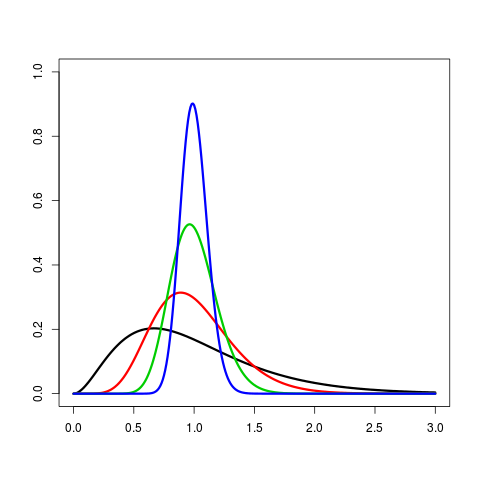
\includegraphics[width=.4\textwidth]{../Figures/FigMixtGamma}
    \end{tabular}
  \end{tabular}


}


%====================================================================
%====================================================================
\section*{Appendix}
{\tiny
  \bibliography{../../../../Biblio/ARC,../../../../Biblio/AST,../../../../Biblio/SSB}
  \bibliographystyle{../../../../LATEX/astats}
  %\bibliographystyle{plain}
  }

%====================================================================
%====================================================================
\end{document}
%====================================================================
%====================================================================


\frame{\frametitle{}
  }

  \vspace{-0.5cm}
  \begin{tabular}{cc}
    \hspace{-0.5cm}
    \begin{tabular}{p{.5\textwidth}}
    \end{tabular}
    &
    \hspace{-1cm}
    \begin{tabular}{p{.5\textwidth}}
    \end{tabular}
  \end{tabular}
